\documentclass[a4paper, 11pt]{article}

\usepackage{a4wide}
\usepackage[latin2]{inputenc}
\usepackage[T1]{fontenc}
\usepackage[english,polish]{babel}
\usepackage{graphicx}
\usepackage{indentfirst}
\usepackage{pgfplots}

\renewcommand{\baselinestretch}{1.5}

\widowpenalty=10000
\clubpenalty=10000

\begin{document}
	
	\thispagestyle{empty}
	\noindent
	Piotr Karoń, 241 626 \hfill Wrocław, dn. 03.04.2019\\
	
	\hfill
	
	\vspace{1cm}
	\begin{center}
		
		\begin{Large}
			\emph{Zadanie projektowe 2.}\\
		\end{Large}
		Badanie efektywności algorytmów grafowych w zależności od rozmiaru instancji oraz sposobu reprezentacji grafu w pamięci komputera.
	\end{center}
	
	\vspace{0.2ex}
	\begin{flushright}
		\begin{minipage}[t]{0.4\columnwidth}
			\noindent
			PROWADZĄCY:\\
			dr Jarosław Mierzwa
		\end{minipage}
	\end{flushright}
	\newpage
	\tableofcontents
	\newpage
	
	\section{Założenia projektowe}
	
	\subsection{Cel}
	\label{sec:cel}
	Celem projektu jest zbadanie efektywności algorytmów Kruskala, Prima, Dijkstry i Bellmana-Forda w zależności od sposobu reprezentacji grafu i wielkości instancji.
	\subsection{Technologie}
	\label{sec:technologie}
	Do implementacji wymienionych struktur użyto języka \textbf{\textit{Kotlin}} w wersji \textbf{\textit{Native}},
	ktĂłra jest kompilowana do kodu maszynowego danej platformy.
	
	\subsection{Przebieg eksperymentu}
	\label{sec:przebieg}
	
	Badania przeprowadzone zostały dla wierzchołków w liczbie: 10, 100, 1000, 10000, 30000,
	dla każdej liczby w gęstościach 25\%, 50\%, 75\%, 99\% osobno dla reprezentacji macierzowej i listowej. Każdy test wykonano 50 razy, a czas uśredniono z wszystkich prób. 
	
	
	\section{KrĂłtki opis algorytmĂłw} 
	\label{sec:ops_struktur}
	
	\subsection{Algorytm Kruskala}
	\label{subsec:tablica}

	Czas działania algorytmu Kruskala dla grafu $G=(V,E)$ zależy od sposobu implementacji zbiorów rozłącznych. W tym projekcie wykorzystano implementację lasu zbiorów rozłącznych z łączeniem według rangi i z kompresją ścieżek.
	
	Całkowity czas działania algorytmu wynosi $O(Elog_2E)$

	\subsection{Lista}
	\label{subsec:lista}
	
	\subsection{Kopiec binarny (maksymalny)}
	\label{sec:kopiec}
	
	
	\section{Wyniki}
	
	\subsection{Wykresy}
	\begin{tikzpicture}[scale=1.4]
	\begin{axis}[
	title = {Średni czas operacji dodawania},
	%title style = { text width 16em},
	xlabel = {liczba elementĂłw},
	ylabel = {czas [ms]},
	xmin = 0, xmax = 5200,
	ymin = 0, ymax = 240,
	legend pos = north west,
	ymajorgrids=true, grid style = dashed
	]
	
	\addplot[color=red, mark=*]
	coordinates{
		(	10	,	0	)
		(	100	,	0	)
		(	200	,	0	)
		(	500	,	1	)
		(	1000	,	2	)
		(	2000	,	4	)
		(   5000, 10 )
		
	};
	\legend{AVL,BST,kopiec,lista,tablica}
	
	\addplot[color=blue, mark=x]
	coordinates{
		(	10	,	0	)
		(	100	,	0	)
		(	200	,	0	)
		(	500	,	0	)
		(	1000	,	1	)
		(	2000	,	2	)
		(	5000	,	6	)
		
	};
	
	\addplot[color=green, mark=+]
	coordinates{
		
		(	10	,	0	)
		(	100	,	0	)
		(	200	,	0	)
		(	500	,	0	)
		(	1000	,	0	)
		(	2000	,	0	)
		(	5000	,	1	)
		
	};
	\legend{kopiec}
	
	\addplot[color=yellow, mark=|]
	coordinates{
		(	10	,	0	)
		(	100	,	0	)
		(	200	,	0	)
		(	500	,	0	)
		(	1000	,	0	)
		(	2000	,	0	)
		(	5000	,	2	)
		
		
	};
	\legend{lista}
	
	\addplot[color=brown, mark=star]
	coordinates{
		(	10	,	0	)
		(	100	,	0	)
		(	200	,	0	)
		(	500	,	2	)
		(	1000	,	9	)
		(	2000	,	36	)
		(	5000	,	216	)
		
	};
	\legend{AVL,BST,kopiec,lista,tablica}
	
	\end{axis}
	
	\end{tikzpicture}
	
	\begin{tikzpicture}[scale=1.4]
	\begin{axis}[
	title = {Średni czas operacji szukania},
	title style = {},
	xlabel = {liczba elementĂłw},
	ylabel = {czas [ms]},
	xmin = 0, xmax = 5200,
	ymin = 0, ymax = 3050,
	legend pos = north west,
	ymajorgrids=true, grid style = dashed
	]
	
	\addplot[color=red, mark=*]
	coordinates{
		(	10	,	0	)
		(	100	,	0	)
		(	200	,	0	)
		(	500	,	0	)
		(	1000	,	0	)
		(	2000	,	1	)
		
		
	};
	\legend{AVL}
	
	\addplot[color=blue, mark=x]
	coordinates{
		(	10	,	0	)
		(	100	,	0	)
		(	200	,	0	)
		(	500	,	0	)
		(	1000	,	0	)
		(	2000	,	2	)
		(	5000	,	4	)
		
	};
	\legend{BST}
	
	\addplot[color=green, mark=pentagon]
	coordinates{
		(	10	,	0	)
		(	100	,	0	)
		(	200	,	2	)
		(	500	,	13	)
		(	1000	,	55	)
		(	2000	,	217	)
		(	5000	,	1287	)
		
		
	};
	\legend{kopiec}
	
	\addplot[color=yellow, mark=triangle]
	coordinates{
		(	10	,	0	)
		(	100	,	1	)
		(	200	,	6	)
		(	500	,	37	)
		(	1000	,	146	)
		(	2000	,	561	)
		(	5000	,	3029	)
		
		
	};
	\legend{lista}
	
	\addplot[color=brown, mark=star]
	coordinates{
		(	10	,	0	)
		(	100	,	1	)
		(	200	,	5	)
		(	500	,	32	)
		(	1000	,	126	)
		(	2000	,	482	)
		(	5000	,	2671	)
		
	};
	\legend{AVL,BST,kopiec,lista,tablica}
	
	\end{axis}
	
	\end{tikzpicture}
	
	\begin{tikzpicture}[scale=1.4]
	\begin{axis}[
	title = {Średni czas operacji usuwania},
	%title style = {},
	xlabel = {liczba elementĂłw},
	ylabel = {czas [ms]},
	xmin = 0, xmax = 5200,
	ymin = 0, ymax = 2000,
	legend pos = north west,
	ymajorgrids=true, grid style = dashed
	]
	
	\addplot[color=blue, mark=*]
	coordinates{
		(	10	,	0	)
		(	100	,	0	)
		(	200	,	0	)
		(	500	,	0	)
		(	1000	,	1	)
		(	2000	,	4	)
		(	5000	,	19	)
		
	};
	\legend{BST}
	
	\addplot[color=green, mark=x]
	coordinates{
		(	10	,	0	)
		(	100	,	0	)
		(	200	,	0	)
		(	500	,	1	)
		(	1000	,	3	)
		(	2000	,	6	)
		(	5000	,	20	)
		
		
	};
	\legend{kopiec}
	
	\addplot[color=yellow, mark=pentagon]
	coordinates{
		
		(	10	,	0	)
		(	100	,	1	)
		(	200	,	5	)
		(	500	,	35	)
		(	1000	,	135	)
		(	2000	,	494	)
		(	5000	,	2512	)
		
	};
	\legend{lista}
	
	\addplot[color=brown, mark=triangle]
	coordinates{
		(	10	,	0	)
		(	100	,	1	)
		(	200	,	5	)
		(	500	,	34	)
		(	1000	,	131	)
		(	2000	,	521	)
		(	5000	,	3185	)
		
	};
	\legend{BST,kopiec,lista,tablica}
	
	\end{axis}
	
	\end{tikzpicture}
	
	\begin{tikzpicture}[scale=1.4]
	\begin{axis}[
	title = {Średni czas operacji dodatkowych BST},
	%title style = {},
	xlabel = {liczba elementĂłw},
	ylabel = {czas [ms]},
	xmin = 0, xmax = 5100,
	ymin = 0, ymax = 15000,
	legend pos = north west,
	ymajorgrids=true, grid style = dashed
	]
	
	\addplot[color=red, mark=*]
	coordinates{
		(	10	,	0	)
		(	100	,	10	)
		(	200	,	42	)
		(	500	,	267	)
		(	1000	,	1063	)
		(	2000	,	4377	)
		(   5000 , 28523)
		
	};
	
	\addplot[color=blue, mark=pentagon]
	coordinates{
		(	10	,	0	)
		(	100	,	5	)
		(	200	,	21	)
		(	500	,	136	)
		(	1000	,	543	)
		(	2000	,	2212	)
		(	5000	,	14639	)
		
	};
	\legend{BST}
	
	\addplot[color=green, mark=triangle]
	coordinates{
		(	10	,	0	)
		(	100	,	10	)
		(	200	,	42	)
		(	500	,	279	)
		(	1000	,	1086	)
		(	2000	,	4497	)
		(  5000, 26293)
		
		
	};
	\legend{usuń + DSW, dodaj + DSW, DSW}
	
	\end{axis}
	
	\end{tikzpicture}
	
	
	\subsection{Tabele}
	
	\begin{table}[h!]
		\label{tab:dodawanie}
		\caption{Wyniki operacji dodawania w milisekundach}
		\begin{tabular}{c|c|c|c|c|c}
			*&Tablica&Lista&Kopiec&Bst&Avl\\ \hline
			10	&	0	&	0	&	0	&	0	&	0	\\
			100	&	0	&	0	&	0	&	0	&	0	\\
			200	&	0	&	0	&	0	&	0	&	0	\\
			500	&	2	&	0	&	0	&	0	&	1	\\
			1000	&	9	&	0	&	0	&	1	&	2	\\
			2000	&	36	&	0	&	0	&	2	&	4	\\
			5000	&	216	&	2	&	1	&	6	&	10	\\
			
		\end{tabular}
	\end{table}
	
	\begin{table}[h!]
		\label{tab:szukanie}
		\caption{Wyniki operacji szukania w milisekundach}
		\begin{tabular}{c|c|c|c|c|c}
			*&Tablica&Lista&Kopiec&Bst&Avl\\ \hline
			10	&	0	&	0	&	0	&	0	&	0	\\
			100	&	1	&	1	&	0	&	0	&	0	\\
			200	&	5	&	6	&	0	&	0	&	0	\\
			500	&	32	&	37	&	0	&	0	&	0	\\
			1000	&	126	&	146	&	0	&	1	&	0	\\
			2000	&	482	&	561	&	0	&	2	&	1	\\
			5000	&	2671	&	3029	&	1	&	6	&	2	\\
			
			
		\end{tabular}
	\end{table}
	
	\begin{table}[h!]
		\label{tab:usuwanie}
		\caption{Wyniki operacji usuwania w milisekundach}
		\begin{tabular}{c|c|c|c|c|c}
			*&Tablica&Lista&Kopiec&Bst&Avl\\ \hline
			10	&	0	&	0	&	0	&	0	&	*	\\
			100	&	1	&	1	&	0	&	0	&	*	\\
			200	&	5	&	5	&	0	&	0	&	*	\\
			500	&	34	&	35	&	1	&	0	&	*	\\
			1000	&	131	&	135	&	3	&	1	&	*	\\
			2000	&	521	&	494	&	6	&	4	&	*	\\
			5000	&	3185	&	2512	&	20	&	19	&	*	\\
			
		\end{tabular}
	\end{table}
	
	\begin{table}[h!]
		\label{tab:bst}
		\caption{Wyniki operacji specjalnych BST}
		\begin{tabular}{c|c|c|c|}
			&	RĂłwnowaĹźenie	&	Usuwanie + DSW	&	Dodawanie + DSW		\\ \hline
			10	&	0	&	0	&	0		\\
			100	&	10	&	10	&	5		\\
			200	&	42	&	42	&	21		\\
			500	&	279	&	267	&	136		\\
			1000	&	1086	&	1063	&	543		\\
			2000	&	4497	&	4377	&	2212		\\
			5000	&	28523	&	26293	&	15005		\\
			
		\end{tabular}
	\end{table}
	
	\section{Podsumowanie}
	
	Zaimplementowane algorytmy nie są optymalne. W większości jednak założona złożoność obliczeniowa sprawdziła się. Najbardziej obciążające były operacje na drzewie BST z wykorzystaniem algorytmu DSW. Równoważenie drzewa po każdym wstawieniu węzła nie jest dobrym pomysłem. Można to robić co kilka, kilkanaście wstawień -- takie niezrównoważenie nie wpłynie bardziej na złożoność w przypadku innych operacji.
	
	
	\newpage
	\begin{figure}
		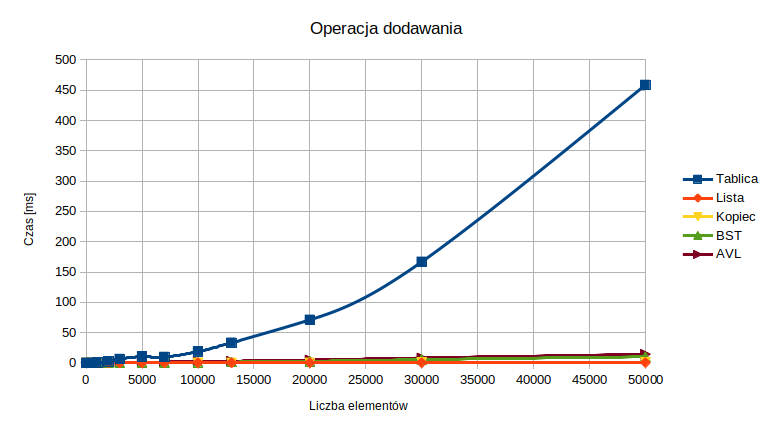
\includegraphics[width=\linewidth]{Wyniki/dodawanie.png}
		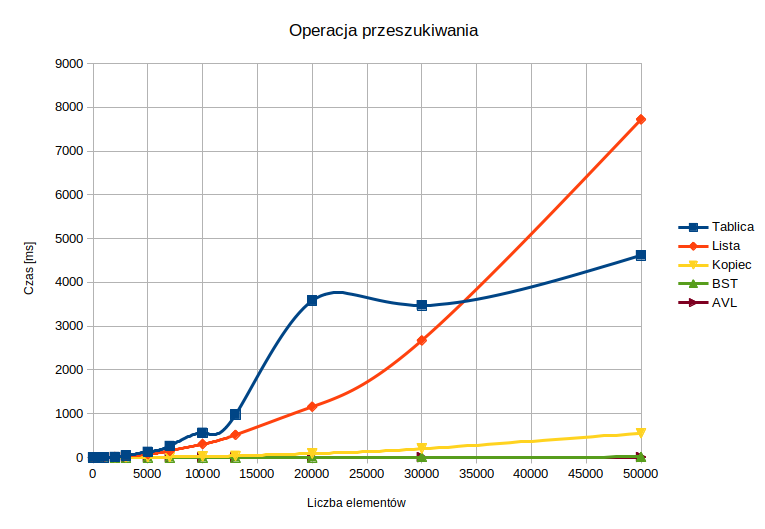
\includegraphics[width=\linewidth]{Wyniki/przeszukiwanie.png}
	\end{figure}
	\begin{figure}
		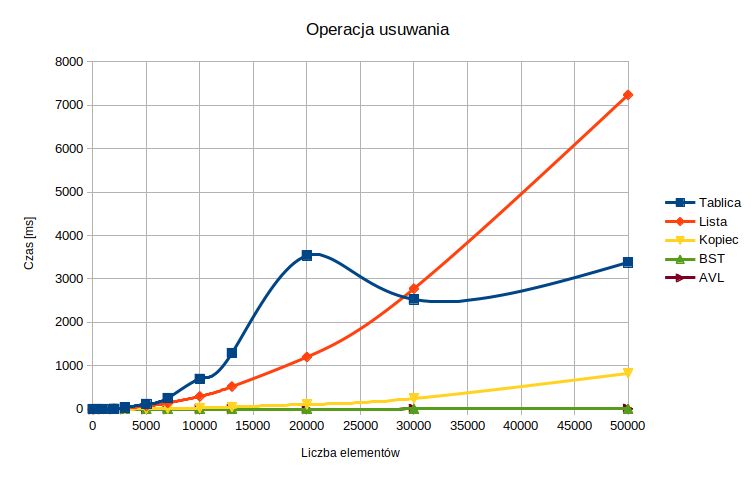
\includegraphics[width=\linewidth]{Wyniki/usuwanie.png}
	\end{figure}
	
	\newpage
	
	\newpage
	%##############################################################
	%##############################################################
	\begin{thebibliography}{99}
		\addcontentsline{toc}{section}{Bibliografia}
		\bibitem{cormen} T. Cormen, C. Leiserson, R. Rivest \emph{Wprowadzenie do algorytmĂłw}, Wydawnictwa Naukowo-Techniczne Warszawa, Wyd. IV, 2004
		\bibitem{cormen-black-red} \cite{cormen} str.  304.
		\bibitem{kaplon} \texttt{tomasz.kaplon.staff.iiar.pwr.wroc.pl/}, strona dr Tomasza Kapłona
		\bibitem{kotlin} \texttt{kotlinlang.org/docs/reference/native-overview.html}, dokumentacja języka Kotlin/Native
		\bibitem{ilotarnow} \texttt{eduinf.waw.pl}, materiały na stronie I LO w Tarnowie
		
		
	\end{thebibliography}
	
\end{document}

%%% Local Variables: 
%%% mode: latex
%%% TeX-master: "sprawozdanie"
%%% End: 
